\begin{frame}[t]
  \frametitle{Perte de Huber}
    {\footnotesize
  \begin{align*}
    L_{\text{Huber}} : \RR \times \RR & \rightarrow \RR \\
    y, f(\xvec) & \mapsto 
                  \begin{cases}
                    \frac{1}{2} \left(y - f(\xvec)\right)^2 & \text{ si } |y - f(\xvec)| < \epsilon \\
                    \epsilon |y - f(\xvec)| - \frac{1}{2} \epsilon^2 & \text{ sinon.} 
                  \end{cases}
  \end{align*}}
   \begin{center}
     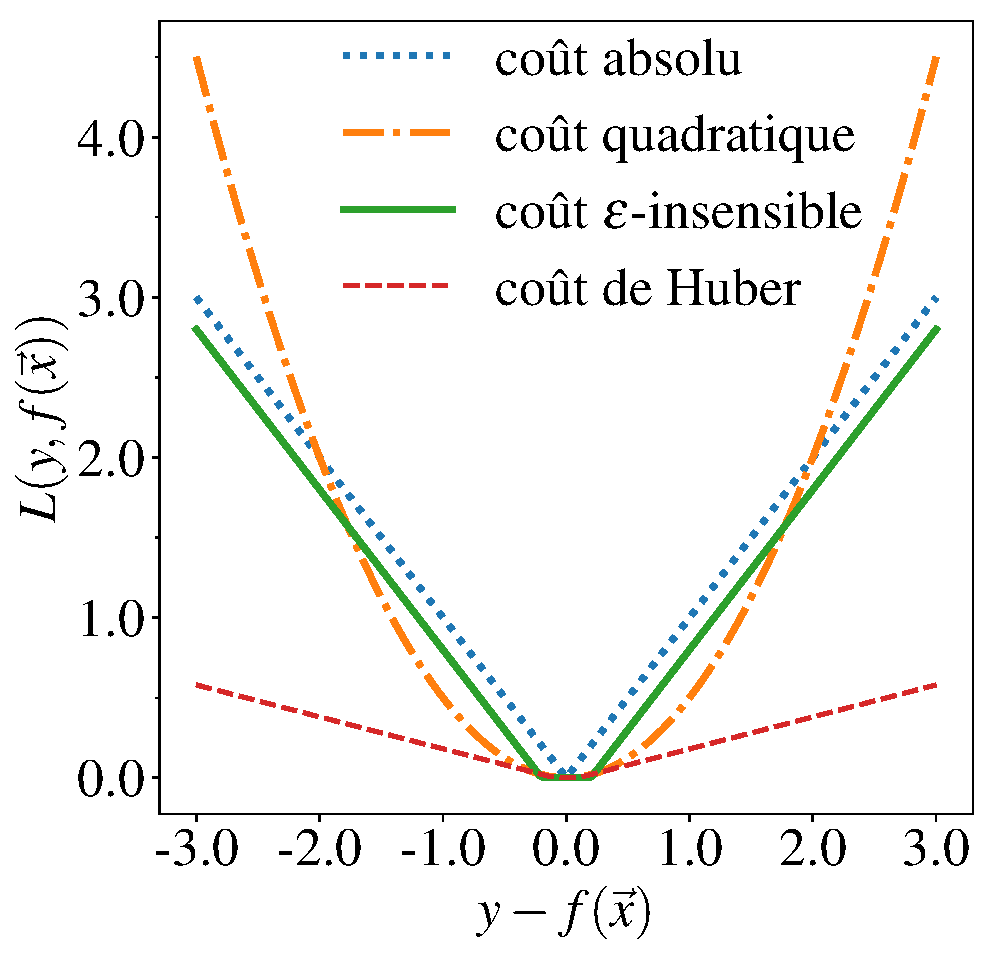
\includegraphics[width=0.5\textwidth]{figures/regression_losses}
   \end{center}
 \end{frame}


\begin{frame}
  \begin{center}
    \red{\LARGE Cours 6 -- Clustering} 
  \end{center}
\end{frame}

\begin{frame}
  \frametitle{Clustering ou partitionnement}
  \begin{itemize}
  \item \red{Clustering :} partitionner les données en sous-ensembles (\red{clusters}) homogènes
  \item Exemples :
    \begin{itemize}
    \item \blue{segmentation de marché}
    \item \blue{communautés} sur un réseau social
    \item \blue{topic modeling} (thématique de textes)
    \item \blue{compression} ou \blue{segmentation d'images}
    \item \blue{sous-types} d'une maladie
  \end{itemize}
  \end{itemize}
\end{frame}

\begin{frame}
  \frametitle{Clustering : Motivation}
  \begin{itemize}
  \item Étude de données \blue{non-étiquetées}
  \item Analyse \blue{exploratoire}
  \item \blue{Visualisation}
  \item Peut précéder une phase d'\blue{inférence} (ex. topic modeling)
  \end{itemize}
\end{frame}


\begin{frame}
  \begin{center}
    \large{1. Évaluation d'un clustering}
  \end{center}
\end{frame}

\begin{frame}
  \frametitle{1.1 Critères géométriques}
  \begin{center}
    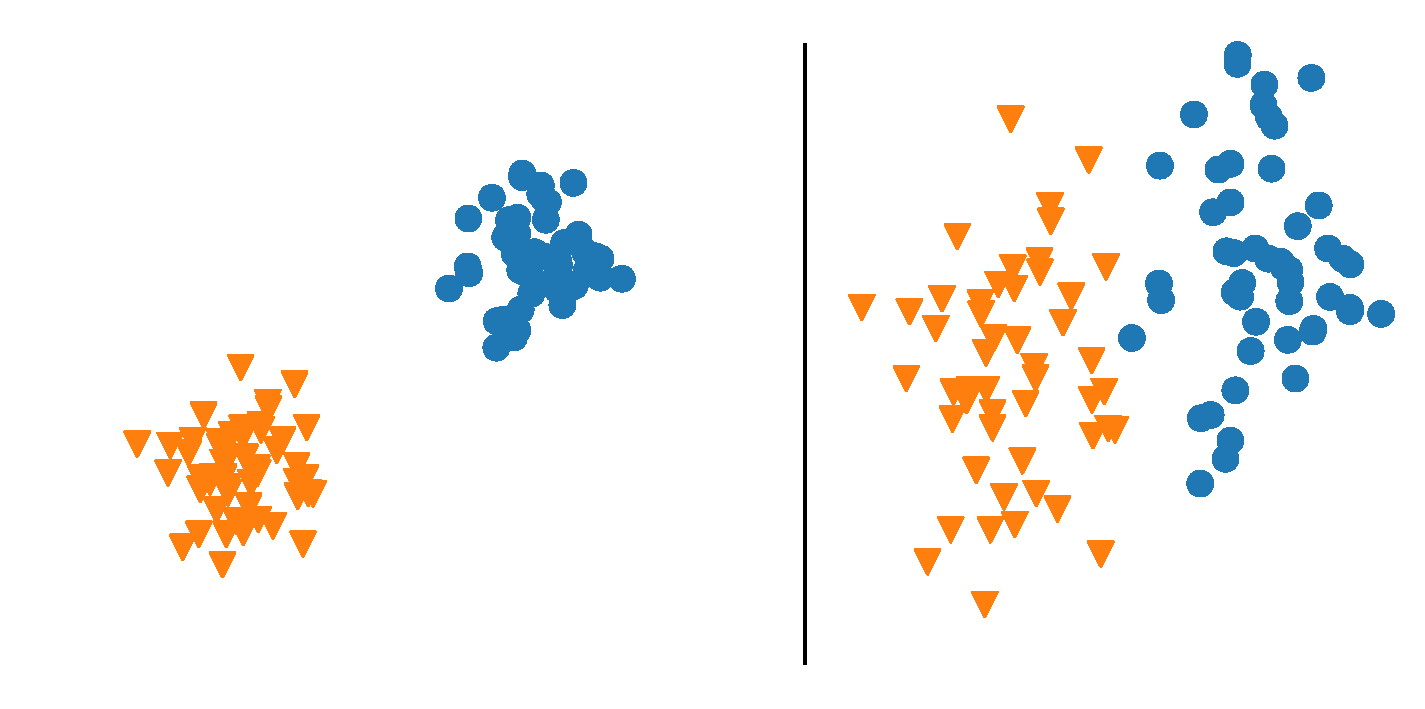
\includegraphics[width=0.5\textwidth]{figures/homogeneity}%
  \end{center}
  \begin{minipage}[t]{0.5\linewidth}
    \begin{itemize}
    \item \red{Homogénéité} \textcolor{gray!70}{(tightness)}
      \begin{itemize}
      \item Pour le cluster $k$ :
        \begin{equation*}
          T_k = \frac{1}{|\cset_k|} \sum_{\xvec \in \cset_k} d(\xvec, \muvec_k)
        \end{equation*}
      \end{itemize}
    \end{itemize}
  \end{minipage}%
  \begin{minipage}[t]{0.5\linewidth}
    \begin{itemize}
    \item \red{Centroïde} du cluster $\cset$:
      \[ \muvec_{\cset} = \frac{1}{\cset}\sum_{\xvec \in \cset}\xvec\]
    \item \red{Médoïde} : l'élément de $\cset$ le plus proche de $\muvec_{\cset}$
    \end{itemize}  
  \end{minipage}
  \begin{itemize}
  \item[]  
    \begin{itemize}
    \item Pour le clustering complet :  $T = \frac1K\sum_{k=1}^{K}T_k$
    \end{itemize}
  \end{itemize}
\end{frame}

\begin{frame}
  \frametitle{1.1 Critères géométriques}
  \begin{center}
    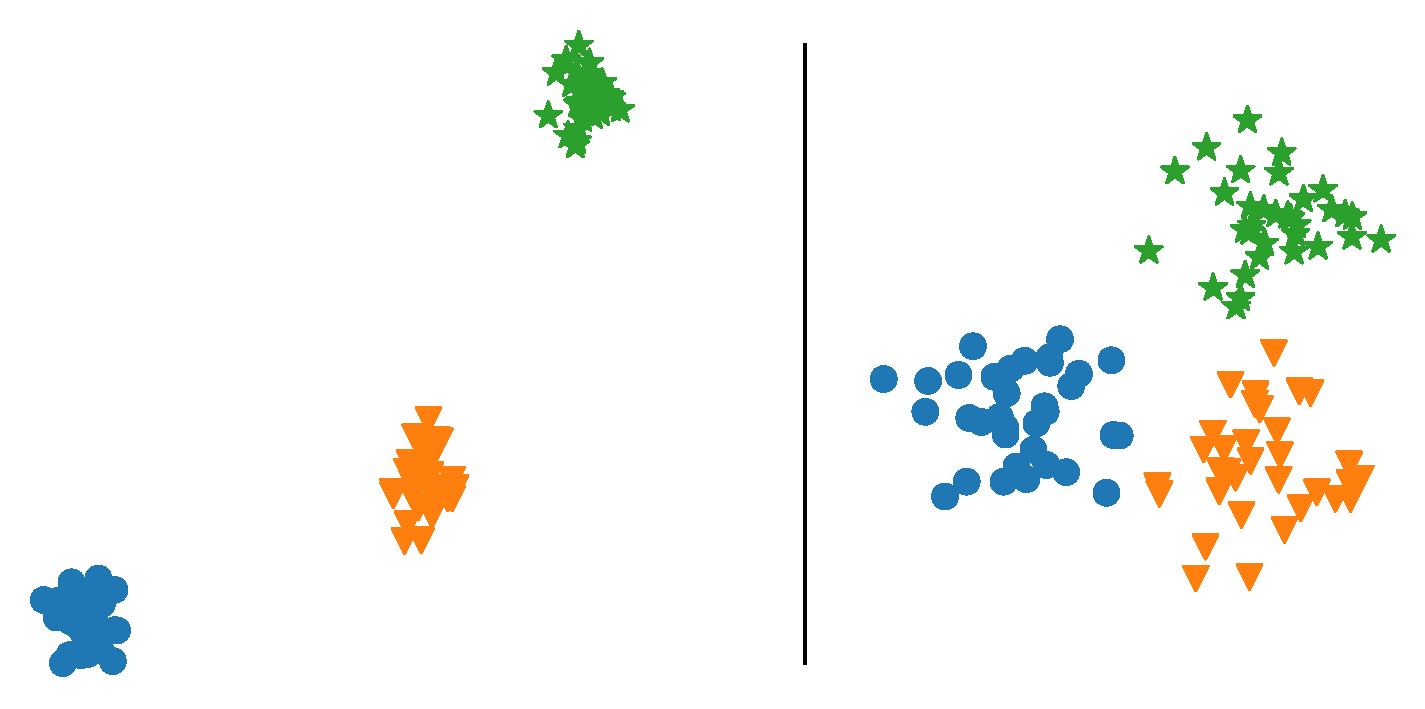
\includegraphics[width=0.5\textwidth]{figures/separability}%
  \end{center}
  \begin{itemize}
  \item \red{Séparabilité}
    \begin{itemize}
    \item Pour les clusters $k$ et $l$ : 
      \begin{equation*}
        s_{kl} = d(\muvec_k, \muvec_l)
      \end{equation*}
    \item Pour le clustering :
      \begin{equation*}
	S = \frac{2}{K(K-1)}\sum_{k=1}^{K-1}\sum_{l=k+1}^{K}s_{kl}
      \end{equation*}
    \end{itemize}
  \end{itemize}
\end{frame}

\begin{frame}
  \frametitle{1.1 Critères géométriques}
  \begin{itemize}
  \item \red{Coefficient de silhouette}
    \begin{itemize}
    \item Pour un point $\xvec$ :
      {\footnotesize
      \begin{align*}
	a(\xvec) & = \frac{1}{|\cset_{k(\xvec)}| - 1} \sum_{\uvec \in \cset_{k(\xvec)}}d(\xvec, \uvec) \\
	b(\xvec) & = \min_{l\neq k(\xvec)}\frac{1}{|\cset_l|} \sum_{u \in \cset_l}d(\uvec, \xvec) \\
        s(\xvec) & = \frac{b(\xvec) - a(\xvec)}{\max(a(\xvec), b(\xvec))}
      \end{align*}}

  \item Pour le clustering :
      \begin{equation*}
        s = \frac1n \sum_{i=1}^n s(\xvec^i).
      \end{equation*}
    \end{itemize}
  \end{itemize}
\end{frame}

\begin{frame}
  \frametitle{1.2 Stabilité des clusters}
    \begin{center}
      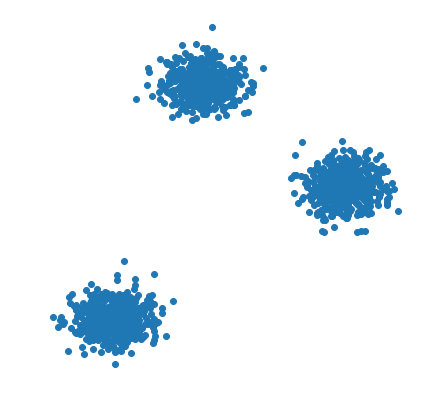
\includegraphics[width=0.7\textwidth]{figures/three_clusters}%
    \end{center}
\end{frame}

\begin{frame}
  \frametitle{1.3 Comparaison à des étiquettes connues}
  \begin{itemize}
  \item Difficulté : les clusters sont numérotés arbitrairement
  \item \red{Indice de Rand}
        \begin{equation*}
      \text{RI} = \frac2{n (n-1)} \sum_{i=1}^n \sum_{l=i+1}^n 
      \indic_{k(\xvec^i) = k(\xvec^l)} \, \indic_{y^i = y^l} + 
      \indic_{k(\xvec^i) \neq k(\xvec^l)} \, \indic_{y^i \neq y^l}.
    \end{equation*}
  \end{itemize}
\end{frame}

\begin{frame}
  \begin{center}
    \large{2. Clustering hiérarchique}
  \end{center}
\end{frame}

\begin{frame}
  \frametitle{Dendrogramme}
  \begin{center}
    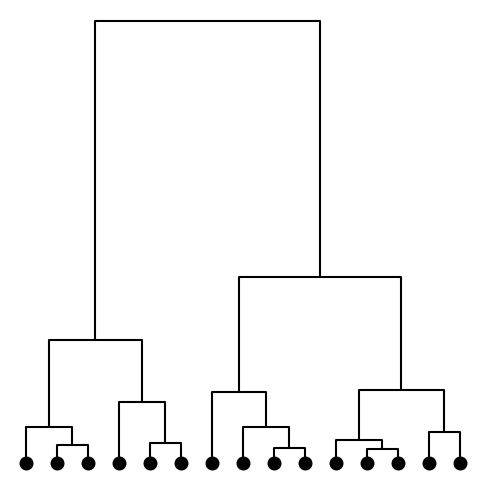
\includegraphics[width=0.7\textwidth]{figures/dendrogram}%
  \end{center}
\end{frame} 

\begin{frame}
  \frametitle{Construction}
  \begin{itemize}
  \item Construction \red{agglomérative} \textcolor{gray!70}{(bottom-up)}
    \begin{itemize}
    \item Initialement : chaque point est son propre cluster 
    \item On fusionne itérativement les clusters les plus proches
    \end{itemize}
  \item Construction \red{divisive} \textcolor{gray!70}{(top-down)}
    \begin{itemize}
    \item Intialement : tous les points sont dans le même cluster 
    \item On sépare itérativement les clusters en deux
    \end{itemize}
  \end{itemize}
\end{frame}

\begin{frame}
  \frametitle{Fonctions de lien}
  \begin{itemize}
  \item \red{Fonction de lien} \textcolor{gray!70}{(linkage)} : distance entre deux clusters
    \begin{itemize}
    \item \red{Lien simple} \textcolor{gray!70}{(single linkage)}
      \[ d_{\text{simple}}(\cset_k, \cset_l) = \min_{(\uvec, \vvec) \in \cset_k \times \cset_l } d(\uvec, \vvec).
      \]
      \pause
    \item \red{Lien complet} \textcolor{gray!70}{(complete linkage)}
      \[
        d_{\text{complet}}(\cset_k, \cset_l) = \max_{(\uvec, \vvec) \in \cset_k \times \cset_l} d(\uvec, \vvec).
      \]
      \pause
    \item \red{Lien moyen} \textcolor{gray!70}{(average linkage)} ou UPGMA \textcolor{gray!70}{(Unweighted Paired Group Method with Arithmetic mean)}
      \[
        d_{\text{moyen}}(\cset_k, \cset_l) = \frac1{\lvert \cset_k \rvert} 
        \frac1{\lvert \cset_l \rvert}
        \sum_{\uvec \in \cset_k}\sum_{\vvec \in \cset_l} d(\uvec, \vvec).
      \]
    \end{itemize}
  \end{itemize}
\end{frame}

\begin{frame}[t]
  \frametitle{Fonctions de lien}
  \begin{itemize}
  \item \red{Fonction de lien} \textcolor{gray!70}{(linkage)} : distance entre deux clusters
    \begin{itemize}
    \item \red{Lien centroïdal} \textcolor{gray!70}{(centroid linkage)}
      \[
        d_{\text{centroidal}}(\cset_k, \cset_l) = d \left (\frac1{\lvert \cset_k \rvert} 
          \sum_{\uvec \in \cset_k} \uvec, 
          \frac1{\lvert \cset_l \rvert} \sum_{\vvec \in \cset_l} \vvec \right) = 
        d(\muvec_k, \muvec_l).
      \]
    \end{itemize}
  \end{itemize}
\end{frame}


\begin{frame}
  \begin{center}
    \large{3. Algorithme des k-moyennes}
  \end{center}
\end{frame}

\begin{frame}
  \frametitle{Variance intra-cluster}
  \begin{itemize}
  \item \red{Variance intra-cluster}
    \[
            \text{Var}_\text{in}(\cset) = \frac1{\lvert \cset \rvert} \sum_{\xvec \in \cset}
      \ltwonorm{\xvec - \muvec}^2.
    \]
  \item Minimiser la variance intra-cluster : créer des clusters \blue{homogènes}
  \end{itemize}
\end{frame}

\begin{frame}
  \frametitle{Algorithme de Lloyd}
  \begin{itemize}
  \item \blue{Initialisation :} choisir les $\muvec_1, \muvec_2, \ldots, \muvec_K$ parmi les données. 
  \item \blue{Affecter} chaque observation $\xvec \in \dset$ au centroïde dont elle est le plus proche :
    \begin{equation*}
      k(\xvec^i) = \argmin_{k=1, \ldots, K}\ltwonorm{\xvec^i - \muvec_k}^2
    \end{equation*}
  \item \blue{Recalculer} les centroïdes $\muvec_k$. 
  \item \blue{Répéter} jusqu'à ce que les affectations ne changent plus. 
  \end{itemize}
\end{frame}

\begin{frame}
  \frametitle{Algorithme de Lloyd}
  \begin{itemize}
  \item \blue{Avantages :}
    \begin{itemize}
    \item Converge rapidement en pratique
    \end{itemize}
    \pause
  \item \blue{Inconvénients :}
    \begin{itemize}
    \item Nécessité de fixer $K$ 
    \item Approche \blue{gloutonne} : pas de garantie de minimum global
    \item \blue{Stochasticité} : dépend de l'initialisation \pause $\rightarrow$ k-means++ 
    \item Clusters nécessairement \blue{convexes} \pause $\rightarrow$ kernel k-means
    \end{itemize}
  \end{itemize}
\end{frame}

\begin{frame}
  \begin{center}
    \large{4. DBSCAN}
  \end{center}
\end{frame}

\begin{frame}
  \frametitle{DBSCAN: Motivation}
  \begin{center}
    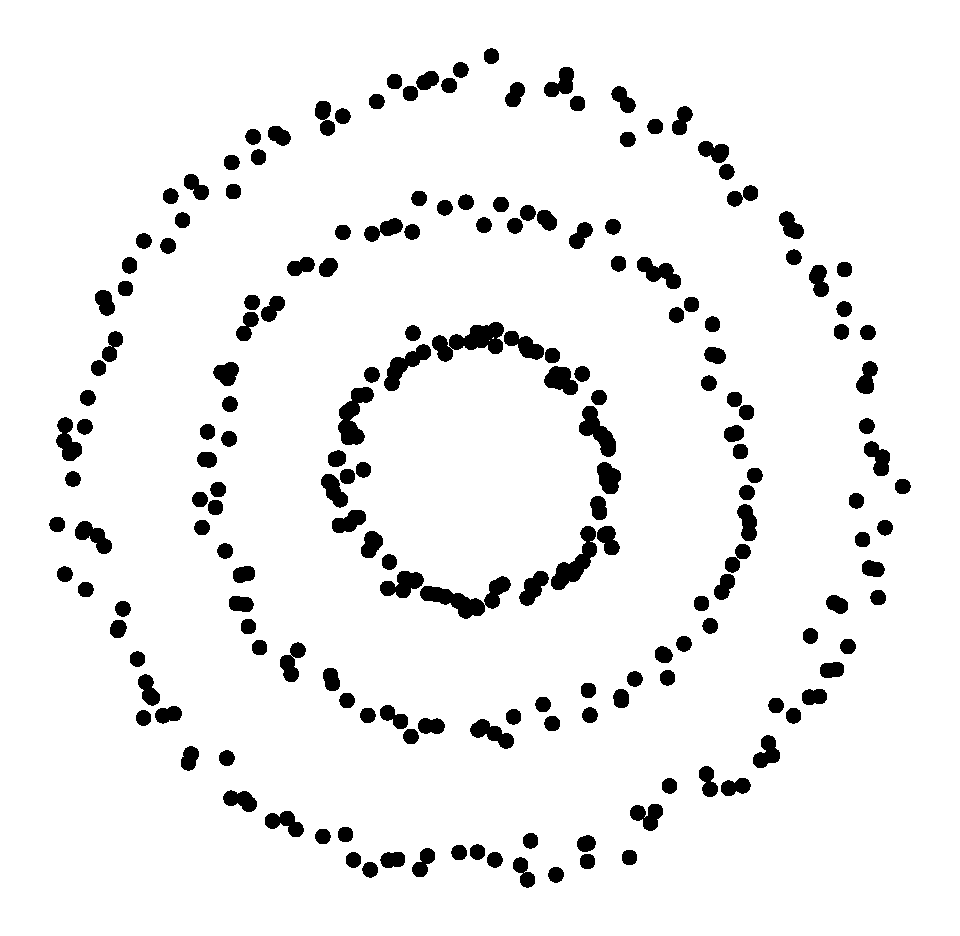
\includegraphics[width=.3\textwidth]{figures/dbscan_pb}%
    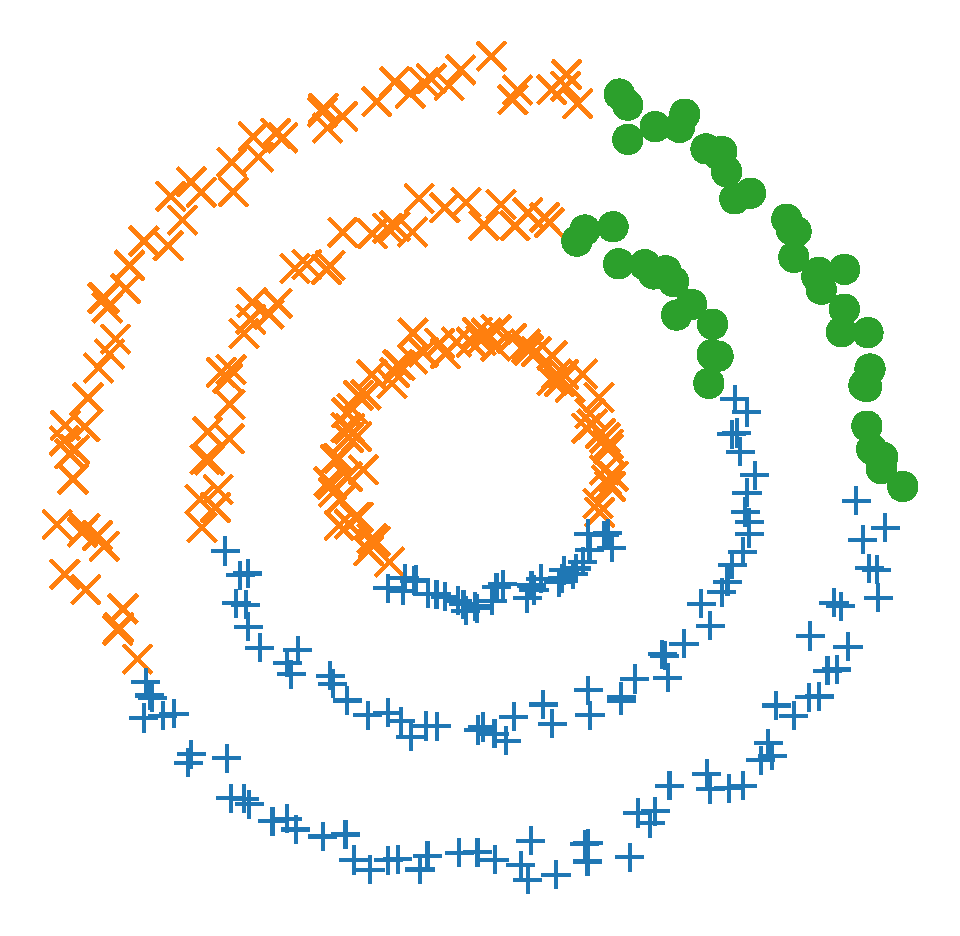
\includegraphics[width=.3\textwidth]{figures/hierarchical_sol}%
    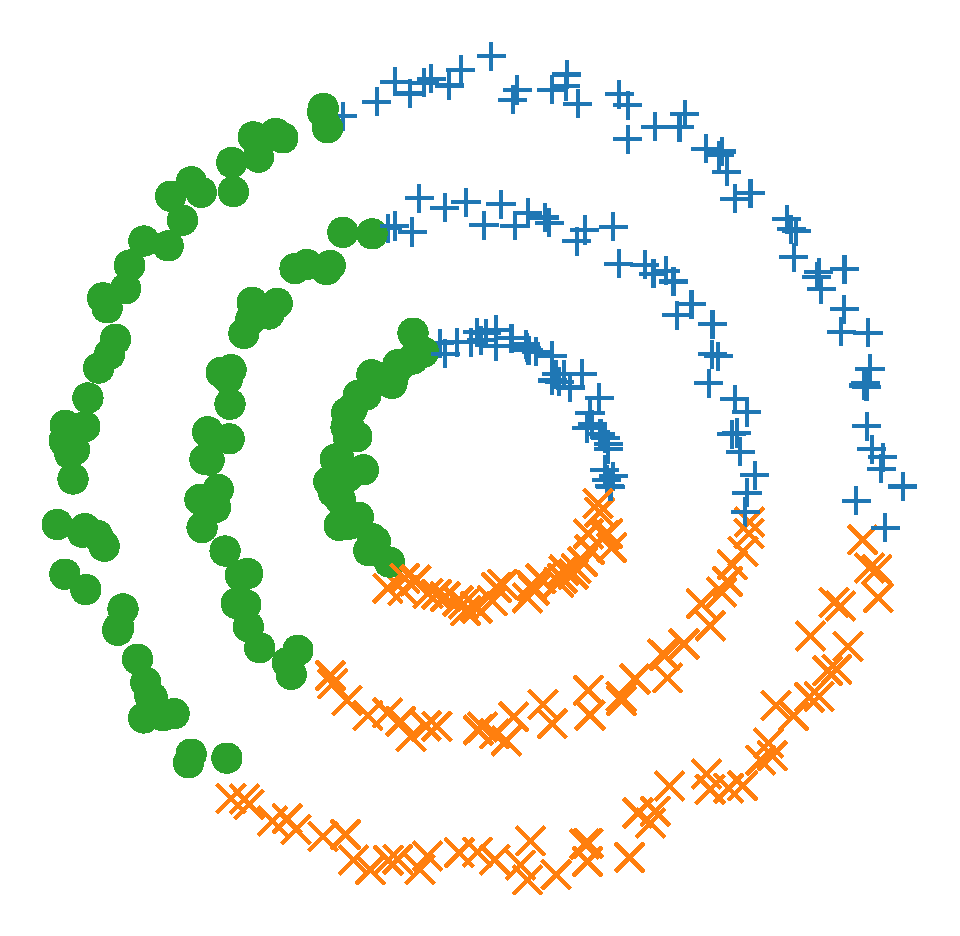
\includegraphics[width=.3\textwidth]{figures/kmeans_sol}
  \end{center}
  \begin{itemize}
  \item Idée : utiliser la \blue{densité}
  \end{itemize}
\end{frame}


\begin{frame}
  \frametitle{DBSCAN}
  \begin{itemize}
  \item Idée : itérer \blue{de proche en proche} par des \blue{voisinages} (boules) de rayon $\epsilon$
  \item Les points \blue{isolés} (min $n_{\min}$ points par cluster) sont du bruit 
  \end{itemize}
  \begin{center}
    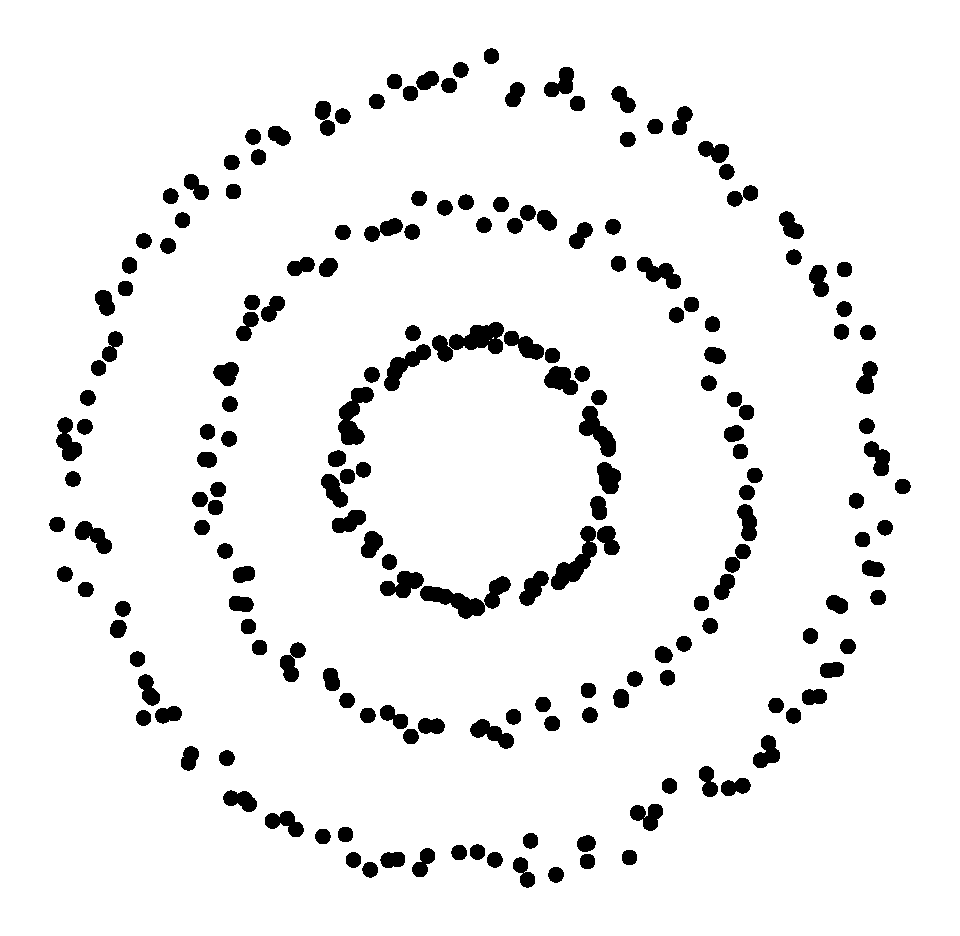
\includegraphics[width=.6\textwidth]{figures/dbscan_pb}
  \end{center}
\end{frame}

\begin{frame}
  \frametitle{DBSCAN : avantages et inconvénients}
  \begin{itemize}
  \item \blue{Avantages :}
    \begin{itemize}
    \item n'impose pas de forme particulière
    \item simple, pas de définition du nombre de clusters
    \item robustesse aux données aberrantes
    \end{itemize}
  \pause
  \item \blue{Inconvénients :}
    \begin{itemize}
    \item ne sait pas gérer des écarts
    \item peu de résultats théoriques
    \item pas applicable en très haute dimension 
    \end{itemize}
  \end{itemize}
\end{frame}


\begin{frame}
  \frametitle{Recap}
\end{frame}

